\chapter{Chess-game analysis}

\section{The game of chess}

Chess is a two-player turn-based strategy game played on a checkered board with bounded dimensions: 64 squares arranged in an 8x8 grid, where each player has a set of initial pieces arranged in a specific order aiming to conquer an specific opponent piece: The King.

In game-theory, Chess is classified in the cluster of games with perfect information in which the players move alternately and the game is not subject to randomization.

The history of chess was firstly documented around 6th Century, although the earliest origins are ambiguous. It is believed that the game's predecessor was originated in India, from where the game spread to Persia. After the Arabic occupation, the game was spread through the Muslim world and to Southern Europe, where it evolved into the current form in the 15th Century ~\cite{murray1913history}.


    \begin{figure}[H]
        \centering
        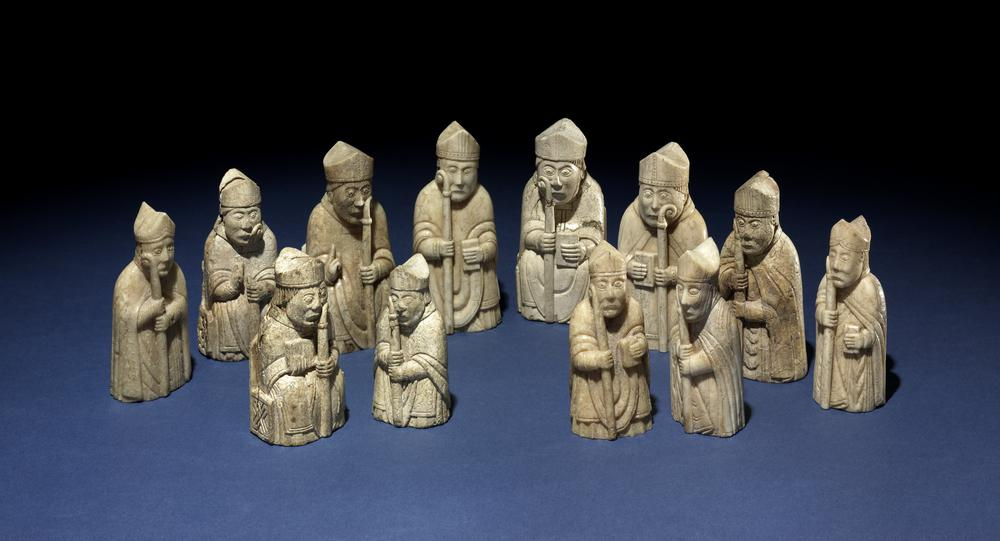
\includegraphics[width=0.6\textwidth]{chessmen}
        \caption{The Lewis chessmen are a group of distinctive 12th-century chess pieces, along with other game pieces, most of which are carved from walrus ivory. Present location: British Museum, London. Image courtesy of Wikipedia Commons}.
    \end{figure}

\section{Computing chess}

\subsection{Zermelo's theorem}

\begin{theorem} 
Zermelo's theorem is a game-theory theorem regarding finite two-person games of perfect information in which the players move alternately and the game is not subject to randomization. It suggests that if the game cannot end in a draw, then one of the two players must have a winning strategy (\textit{i.e. force a win}). 

An alternate statement is that for a game meeting all of these conditions except the condition that a draw is not possible, then either the first-player can force a win, or the second-player can force a win, or both players can force a draw. ~\cite{schwalbe2001zermelo}. 
\end{theorem}

\begin{remark}
As the chess is a finite two-person games of perfect information in which the players move alternately and the game is not subject to randomization, Zermelo's Theorem can be applied for this game. It states that either White can force a win, or Black can force a win, or both sides can force at least a draw.
\end{remark}

With this background of theoretical work, we can state that there must be a perfect algorithm for chess, at least for one of the two players.

\begin{remark}
All endgames of 6 pieces or less have been perfectly solved.
\end{remark}

\begin{remark}
Previous results show that the game of Losing Chess is a win for White. ~\cite{watkins2017losing}. The "losing-winning" move is \textbf{e3} for White.
\end{remark}


\subsection{Chess complexity using Bachmann-Landau notations}

This subsection will present another example of inappropriate use of Bachmann-Landau asymptotic notations for algorithms that do not generalize well. As previously stated, a perfect algorithm for chess exists, even though the state space that it would have to search would be huge. 

Due to finite-bounds of the game and the existence of the 50-move rule, which allows either player to claim a draw if 50 or more moves take place without movement of a pawn  or a piece-capture, based on FIDE-game rules, the longest chess game could be up to 4851 moves. A wide estimation would be counting the total number of possibilities for a the player to move one of (at most) 16 pieces: 8 pawns, each with at most 3 moves, 2 rocks each with at most 14 moves, 2 knights 8 each with at most, 2 bishops, each with at most 14 moves, 28 for a queen and 8 for a king, for a total of 132 possible moves. Definitely these are just hypothetical situation analyzing the worst-case scenario, as in real games the possibilities are far smaller.

Hence, the total number of chess games would be at most $132^{4851}$. (a more realistic estimation would be $10^{500}$)

As a finite game can be simulated in constant time, the above estimation, translated in Bachmann-Landau notations for complexity classes, this means that the perfect algorithm for chess should perform in $O(132^{4851})$. Using the properties of Big-O complexity class, we can state that this algorithm will perform in constant time, with $O(1)$ complexity as this number of total number of chess, regardless how big it is, is still a constant. 

In this situation, the Bachmann-Landau asymptotic notations did not provide useful information and the reason is simple: these notations were developed for asymptotic-scaling problems and algorithms, w/o awareness of discrete values. Even though in most cases these notations were helpful, this is probably not the case in this scenario.

\subsection{Previous work}
Claude Shannon had studied the implications of a brute force solution for solving chess back in the 1950 ~\cite{shannon1950xxii}, when he introduced the \textbf{Shannon number}, a conservative lower bound of the game-tree complexity of chess. The purpose was to validate that any perfect chess algorithms based on brute-force are impractical.

The Shannon number proposed back in 1950 was $10^{120}$, taking into consideration a typical game  of 80 moves at a rate of $10^3$ possibilities for each pair of white-black moves.

Previous work of Claude Shannon was building the foundation of information theory with a landmark paper (1948), \textit{"A Mathematical Theory of Communication"}. 

Further work showed that, based on an average branching factor of 35 and an average game length of 80, the lower bound for the chess game-tree is around $10^{123}$. Victor Allis: ~\cite{allis1994searching}

\section{Chess in r-Complexity}
As we previously stated, the perfect algorithm for chess is part of the $O(1)$ complexity class, as its input values are finite-bounded. Thus, the associated r-Complexity class would be $O_{1}(c)$, where $c$ in a real finite constant. A human-driven calculus of r-Complexity is not feasible, as there are various run-time aspects that are difficult to be taken into consideration and an exact calculus would imply a even greater effort than solving straightforward the chess problem. Thus, we propose an automatic estimation for this algorithm, that has its Bachmann–Landau Complexity known.

The first step was acquiring data on few game-simulation. Using gym framework, we tracked the time-complexity for various number of episodes with different number of steps per each episodes.

    \begin{figure}[H]
        \centering
        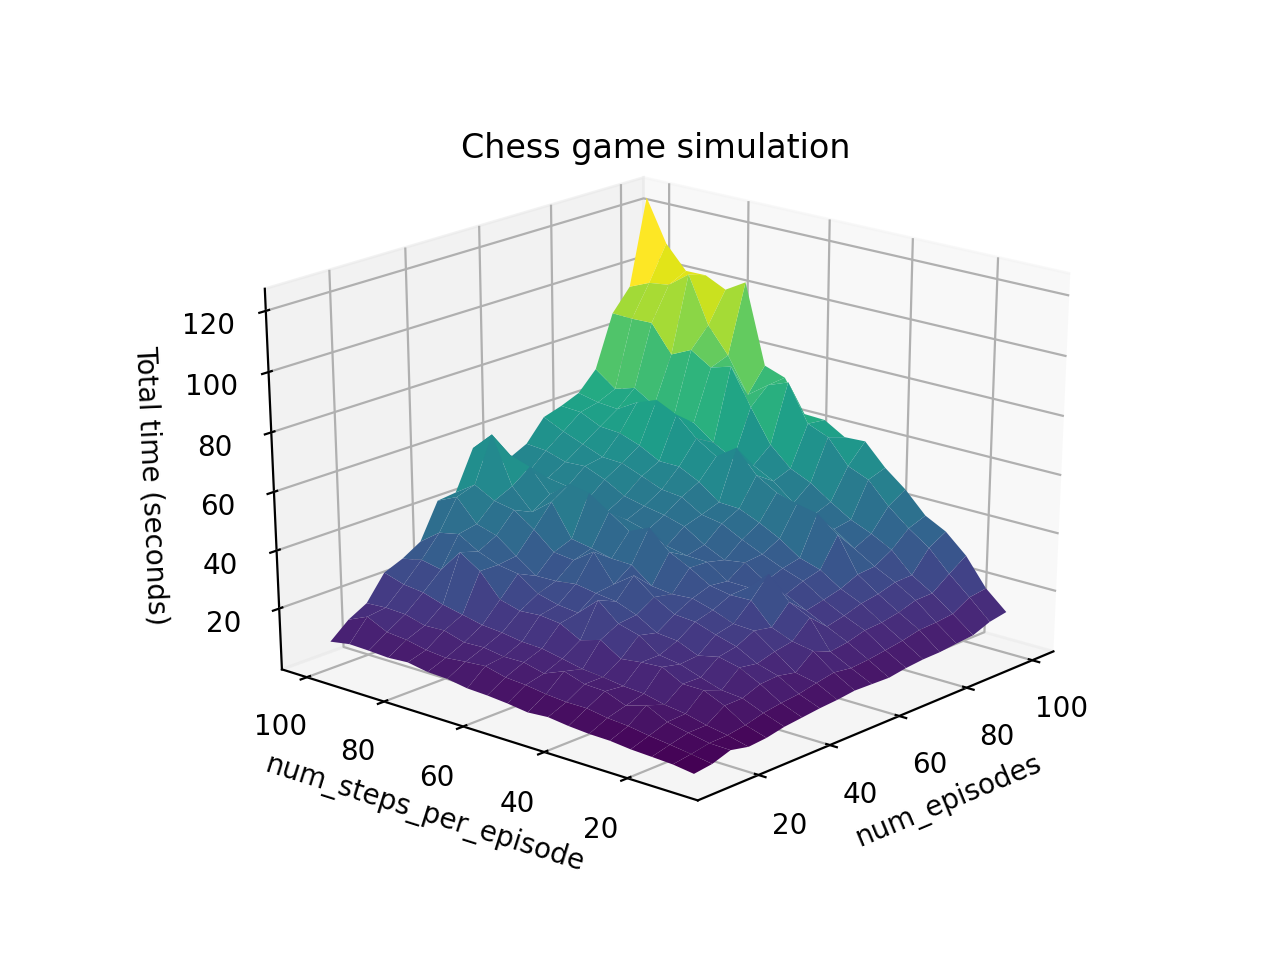
\includegraphics[width=1\textwidth]{chesssim}
        \caption{The plot shows the total computing time based on the variation of parameters corresponding to the total number of games and the average length of a game. Results gathered on a 2.3 GHz Intel Core i5 processor using a serial implementation in Python, using Gym framework. }
    \end{figure}

Using an average game length of 80, the chess-solving problem becomes a one-parameter problem that involves the total number of episodes to be generated. This value is lower-bounded by the value of $10^{123}$. A brute-force solution for this algorithm would act almost linearly in terms of number of episodes to be generated.

    \begin{figure}[H]
        \centering
        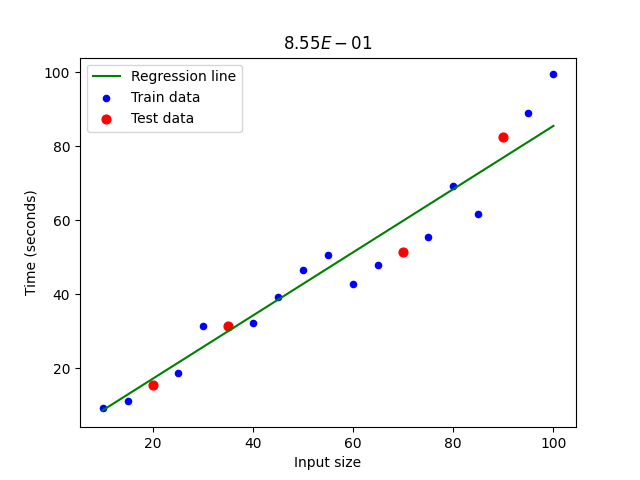
\includegraphics[width=0.7\textwidth]{chesslin}
        \caption{The relationship between the total time required to generate a specific number of games appears to be linear (actual results obtained for an average game length of 80)}
    \end{figure}
 
Of course, many optimization can reduce the total time by even two orders of magnitude. Regardless of the optimization process, for an input of $10^{123}$, the total estimated time using this algorithm would be $0.855 \cdot 10^{123}$ seconds and thus the r-Complexity would be $O_{1}(0.855 \cdot 10^{123} \cdot HZ)$, where $HZ \approx 2.3 \cdot 10^9$.

Such a huge time limit is a result of the greatness of the lower bound for chess. Recall that this is by over 40-orders of magnitude greater that the total estimated number of atoms in the universe.

\subsection{The dream of the perfect algorithm}
All means of computing in 2020 are at an enormous gap from what it would be needed in order to find the perfect algorithm of chess using brute-force solutions. 

Based on the estimated r-Complexity (i.e. $O_{1}(0.855 \cdot 10^{123} \cdot HZ)$, where $HZ \approx 2.3 \cdot 10^9$) we present few scenarios describing what it would take to compute:
\begin{enumerate}[label=\roman*]
  \item \textbf{Scenario 1} 
  
  Assume that each atom in the universe is the state-of-the-art computing core of a modern processor, that operates at a frequency of 5GHz. Assume that the perfect algorithm of chess defies Amdahl's Law by assuming a theoretical unbounded speedup in the latency of the execution. Assume we have 0 latency between inter-process communication. So far, we built an system consisting of $10^{80}$ (this is, the estimate the total number of fundamental particles in the observable universe) computing units operating at $HZ_0 \approx 5 \cdot 10^9$, with zero latency that needs to solve an algorithm with associated complexity of $O_{1}(0.855 \cdot 10^{123} \cdot 2.3 \cdot 10^9)$. That is, assuming perfect distribution and zero overhead, each unit would require approx $10^{42}$ seconds. This is far greater than any estimation of the universe lifespan.
  \item \textbf{Scenario 2} 
  
  Moore's law might come to rescue the hope. Ignoring any physical consideration of the minimum MOSFET scaling process, one might assume that the law might scale indefinitely (even though even Gordon Moore himself foresaw that the rate of progress would eventually reach saturation). 
  
Assume that, the number of transistors in an integrated circuit doubles about every two years and this results in doubling of the transistors implies a doubling in the computing power as well. (ignore the total amount of energy spent and all other considerations). Say that, if today a computing unit would solve the problem in $0.855 \cdot 10^{123}$ seconds, in two-year times, the new computing unit would solve the problem in $\dfrac{0.855 \cdot 10^{123}}{2}$.
  
Similarly, in four-year times, the new unit would solve the problem in $\dfrac{0.855 \cdot 10^{123}}{2^2}$ and in six-year times, it would solve the problem in $\dfrac{0.855 \cdot 10^{123}}{2^3}$. This decrease in time is logarithmic and, theoretical, it reaches after $2 \cdot log_{2}(0.855 \cdot 10^{123})$ years to a point in which the total time for solving chess would be just under 1 second. 

That is, if Moore's law would scale indefinitely, after 816 years, we would be able to solve by brute-force, the game of chess. However, this would also mean that the system would require $2^{408}$ more transistors than the current number of transistors in modern computers (tens of billions), reaching a peak number of transistors of $10^{132}$. 

Unless each fundamental particle in the observable universe could act as $10^{52}$ MOSFET-transistors, this scenario is impracticable.

  \item \textbf{Scenario 3} 
  
  A new, groundbreaking technology appeared and computing is no longer an issue. The algorithm would still require to store at least $10^{123}$ games. Assume the most efficient compression, even though unfeasible, each unique position can be stored by only one brand new memory unit. This would mean that each atom in the universe should be able to store at least $10^{43}$ storing units. This appears to be pretty difficult.
\end{enumerate}

We could further extend our philosophical discussion with many more scenarios, but the point is clear. Perfectly solving the game of chess is a problem far to complicated. And yet, we, as humans, with limited computing power, can naturally play the game of chess charmingly well.